\documentclass[letterpaper,12pt]{article}
\usepackage{graphicx}
\usepackage[margin=1in,letterpaper]{geometry}
\usepackage[final]{hyperref}
\usepackage[capitalise]{cleveref}

\begin{document}
	\begin{titlepage}
		\title{Sample Report: \\Recursive Powers of the Silver Ratio}
		\author{A. Author}
		\date{\today}
		\maketitle
		
		% Do not count the title page for page numbering
		\thispagestyle{empty} 
		% Put abstract on the bottom of the title page
		\vfill
		\begin{abstract}
			\textit{Concise explanation of the experiment, its major findings and their meaning. This is what most people will read and should help them to judge quickly whether your report/paper is of interest to them. Usually, this is not longer than 300 words.}
			
		 	The powers of the silver ratio were calculated using a recursive function and compared to the values produced by the \texttt{cmath} library, which acted as a reference. It was found that due to the limited accuracy of the standard data types, round-off errors accumulate quickly, leading to the recursive function returning false results. After 20 and 40 iterations for single and double precision respectively, this leads to diverging solutions for the silver ratio as one of the roots of the recursive function is smaller than one while the other is greater than one.
		\end{abstract}
	\end{titlepage}
	
	
	\section{Introduction}
		\textit{This section should put the specific experiment and its significance in a wider context. Assume that the reader has the same level of education as yourself, but does not work in your specific field.}
		
		Recursive functions call themselves with a new input until a certain condition is satisfied. A common example would be the calculation of a single value, where the function exits its cycle when the error on that value reaches a satisfactory level. This can be very useful since recursive functions are comparably easy to write and are usually fairly short resulting in a small program size. However, it can be shown that since the function takes its own output as input, a small error could in fact be amplified by accumulation of round-off errors. The property of whether a function will converge or not is called stability.\cite{numrecinc}
	
	\section{Theory}
		\textit{Provide the theoretical background for your work, such as equations and previous work you are building on. Long derivations, etc. can be put in the appendix, although this section has to contain everything the reader needs to follow the rest of the report.}
		
		Numerical stability in the context of recursive functions is a measure of the round-off error of input data relative to the error of the final result. In other words it shows whether a recursive function converges to a single value or diverges from it. This property of recursive functions can be determined by examining the roots of the equation used. If any of its roots has an absolute magnitude greater than one the recursion is said to be unstable. This means that the function might not converge for small initial errors, which always exist in floating point numbers.\\
		
		In this experiment the characteristic equation used for the recursion relation was
		\begin{equation}
		\phi^{n+1} = \phi^{n-1} - \phi^{n} \indent . \label{recrel}
		\end{equation}
		The roots can be found by factorising $\phi^{n-1}$ out of \cref{recrel}:
		\begin{equation}
		(\phi^{n-1})(\phi^{2} + \phi -1) = 0
		\end{equation}
		The first root is therefore given by $\phi_{1}=0$. The other roots can be found by solving
		\begin{equation}
		\phi^{2} + \phi -1 = 0 \indent , \label{chareq}
		\end{equation}
		which can then be found to be
		$$\phi_{2}=\frac{-1+\sqrt{5}}{2} \indent\indent 
		\phi_{3}=\frac{-1-\sqrt{5}}{2} \indent ,$$
		where $\phi_2$ is also known as the Silver Ratio. The powers of the Silver Ratio can thus be calculated recursively using \cref{recrel}.
		
	\section{Experimental Procedure}
		\textit{Explain the setup of your experiment and how it was carried out in a "repeatable" fashion. This should include a schematic of the main parts of the experiments as well as a flowchart detailing how results were generated. In pure software/simulation experiments, this is just the structure/main features of the simulator and any input provided to it. This section may include preliminary results showing the functionality of the apparatus, but in general it should not present the actual results, just how you generated them.}
	
		A C++ program was written to calculate the powers of the silver ratio. The reference value was calculated using the \texttt{pow} function available in the \texttt{cmath} library in double precision. Furthermore the powers were calculated both in \texttt{float} and \texttt{double} using \cref{recrel} as a recursive function, shown in \cref{fig:function}. The obtained data was written to a text file and plotted using matplotlib for Python.
		
	\begin{figure}[h]
		\centering
		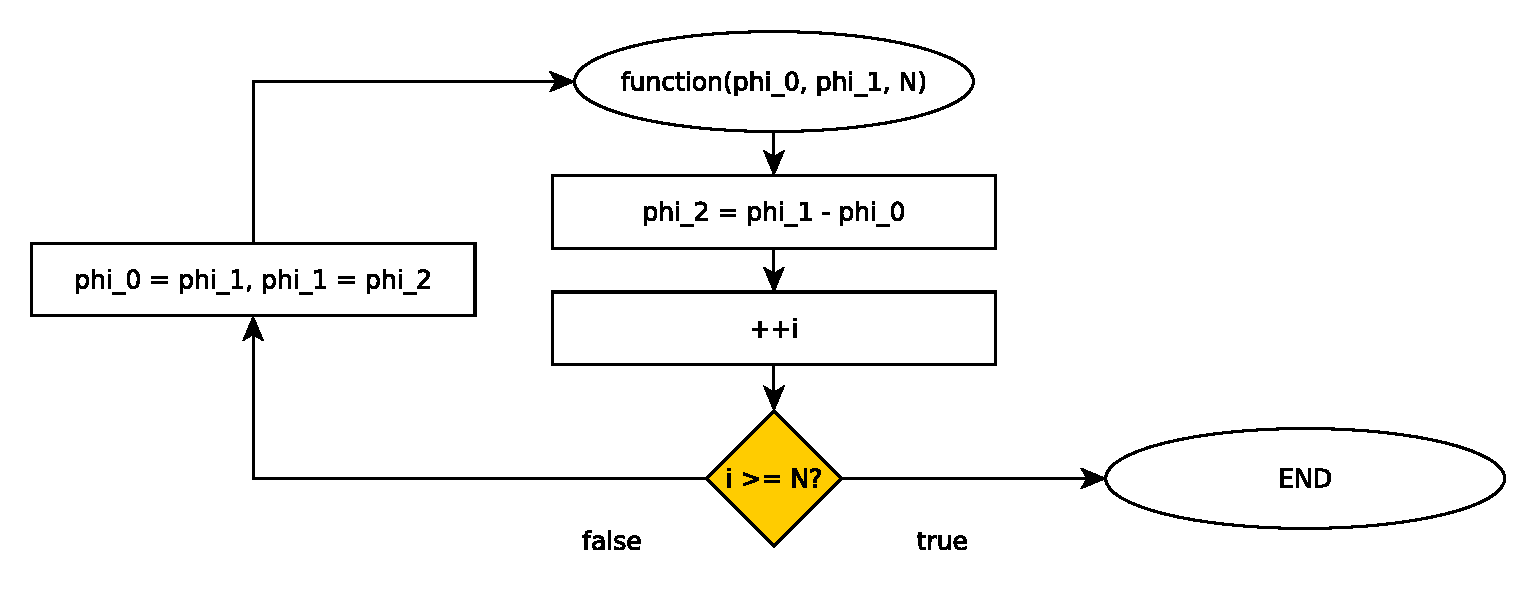
\includegraphics[width=0.65\textwidth]{flowchart.pdf}
		\caption{Flowchart of the recursive function used to calculate the silver ratio. N is the power of the number to be calculated.}
		\label{fig:function}
	\end{figure}
	
	
	\section{Results and Discussion}
		\textit{Here you present your results and explain their meaning. Graphs are usually better than presenting plain numbers since any trend, scaling, etc. can be easily spotted by the reader.
			This section also includes the discussion of errors compared to theoretical values or earlier research, which includes the calculation of errors and an explanation for the sources of these errors. If there are extensive intermediate results, they may be put into the appendix with only the final values appearing here.}
	
	\begin{figure}[h]
		\centering
		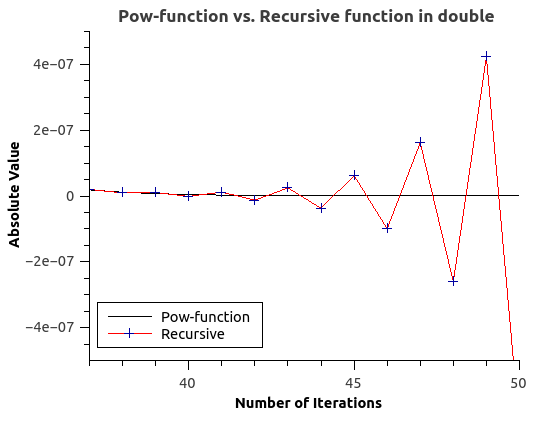
\includegraphics[width=0.45\textwidth]{powvsdouble.png}
		\caption{Exponential growth of the error amplified by the recursive function.}
		\label{fig:powvsrec}
	\end{figure}
	
	On examining the output, it was found that the recursively calculated values diverged from the reference given by the \texttt{pow} function as the exponent increased. This can be explained by the stability of the function used. Since one of the roots has a magnitude greater than 1, the function is by definition unstable. For the investigated relation this means that one of the non-zero roots grows faster than the other. While the powers of $\phi_2$ decrease exponentially in their value, the powers of $\phi_3$ increase exponentially. This means that even the slightest offset in the initial definition of the silver ratio will grow exponentially as can be seen in \cref{fig:powvsrec}. \\
	
	\begin{figure}[h]
		\centering
		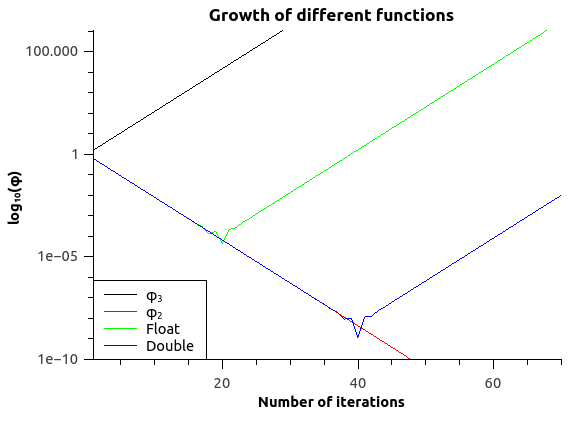
\includegraphics[width=0.55\textwidth]{growth.png}
		\caption{Magnitude of float and double powers compared to reference values $\phi_2$ and $\phi_3$}
		\label{fig:growth}
	\end{figure}
	
	Although the initial offset is only around $10^{-15}$ for double precision, the error becomes larger than the value itself after roughly 40 iterations. This behaviour is, as expected, even more extreme for single precision floating point numbers, where the error reaches this point after only 20 iterations. \cref{fig:growth} shows this behaviour comparing the growth rates of different initial guesses to the reference values calculated by the \texttt{pow} function.
	It demonstrates quite clearly how the values calculated by the recursive function initially follow the growth of their start value, then oscillate around the true value and then start to grow at the rate of the other root.
	
	
	\section{Conclusions}
		\textit{This section will put your findings into greater context and highlight major findings and their meaning for the scientific community. It might also hint at possible extensions, future work, etc. This is what most people will read beyond the abstract.}
	
		It has been shown that the use of recursive functions can create problems in computing due to the limited precision numbers can be stored with. If a function used for a recursion fulfils instability criteria, namely having at least one root with a magnitude greater than one, instability limitations have to be taken into consideration. For the case of the silver ratio, especially using double precision, errors only became catastrophic after 40 iterations, although they are measurable from the first iteration. This occurs much earlier using single precision: after 20 iterations in this case. A possible test to see if a program using double precision is affected may be to use single precision and to examine possible discrepancies.
	
	% The references will be created using the following commands.
	% Make sure you put the references in the order of their appearance in the text.
	% If you need many references and change the order of appearance in the text often, it is better to use bibtex as it will handle this automatically
	\begin{thebibliography}{99}
		
		\bibitem{numrecinc}
		W.~H. Press, S.~A. Teukolsky, W.~T. Vetterling, and B.~P. Flannery, {\em
			Numerical Recipes in C}.
		\newblock The Pitt Building, Trumpington Street, Cambridge CB2 1RP: Press
		Syndicate of the University of Cambridge, 2nd~ed., 1992.
		
	\end{thebibliography}
	
	
\end{document}